% ANL Beamer template
\documentclass[aspectratio=169]{beamer}
\usepackage[english]{babel}
\usepackage[utf8]{inputenc}

% AMSLaTeX packages
\usepackage{amsthm}
\usepackage{amsmath}
\usepackage{amsfonts}
\usepackage[algoruled]{algorithm2e}

\usetheme{default}
\useoutertheme{default}
% we want to use images
\usepackage{graphicx}
\usepackage{movie15}
\usepackage{hyperref}

% table relates packages
\usepackage{booktabs}
\usepackage{multirow}
% pick a font
\usepackage{palatino}           
% \usepackage{times}
\usepackage{tikz}
\usetikzlibrary[positioning,arrows,decorations.pathmorphing,backgrounds,fit,calc]
% \AtBeginSection[]  % "Beamer, do the following at the start of every section"
% {
%   \begin{frame}<beamer> 
%     \frametitle{Outline} % make a frame titled "Outline"
%     \tableofcontents[currentsection]  % show TOC and highlight current section
%   \end{frame}                    
% }

% \AtBeginSubsection[]
% {
%   \begin{frame}
%     \frametitle{Outline}
%     \tableofcontents[currentsection,currentsubsection]
%   \end{frame}
% }

\AtBeginSection[]
{
   \begin{frame}
       \frametitle{Outline}
       \tableofcontents[currentsection]
   \end{frame}
}

\newcommand{\ebox}[1][1em]{\framebox[#1]{\phantom{M}}}

\setlength\arraycolsep{1.4pt}% some length

%gets rid of navigation symbols
\setbeamertemplate{navigation symbols}{}

%gets rid of bottom navigation bars
\setbeamertemplate{footline}[page number]{}
\setbeamertemplate{headline}{}


\usebackgroundtemplate{\includegraphics[width=\paperwidth]{../templates/NormalANLBlue}}

% Define big arrow down
\newcommand{\xdownarrow}[1]{%
  {\left\downarrow\vbox to #1{}\right.\kern-\nulldelimiterspace}
}

% Packages used
\usepackage{xcolor,ulem}
\usepackage{listings}
% Define custom style for Python code listings
\definecolor{codegreen}{rgb}{0,0.6,0}
\definecolor{backcolour}{rgb}{0.95,0.95,0.92}
\lstdefinestyle{python}{
    language=python,
    numbers=none,
    backgroundcolor=\color{backcolour},
    commentstyle=\color{blue},
    keywordstyle=\color{magenta},
    stringstyle=\color{codegreen},
    basicstyle=\ttfamily\scriptsize,
    breakatwhitespace=false,
    breaklines=true,
    captionpos=b,
    keepspaces=true,
    showspaces=false,
    showstringspaces=false,
    showtabs=false,
    tabsize=3
}

% Title/author info
\title{\bigskip
\\
Exploiting structures in multiobjective simulation optimization problems}
\author{Tyler Chang$^a$ and Stefan Wild$^{a\rightarrow b}$}
\institute{$^a$Mathematics and Computer Science Division,\\
Argonne National Laboratory\\

\medskip

$^b$Applied Mathematics and Computational Research Division,\\
Lawrence Berkeley National Laboratory}
\date{SIAM OP 23}

% Slides start here
\begin{document}

% Set the background graphics
\setbeamertemplate{footline}{}
{
\usebackgroundtemplate{\includegraphics[width=\paperwidth]{../templates/TitleANLBlue}}
\frame{\titlepage}
}
\setbeamertemplate{footline}[page number]{}

% FRAME: overview
\begin{frame}
  \frametitle{Outlines}
  \tableofcontents
\end{frame}

% ========================================
% main slides come here
% ========================================

\section{Intro, ParMOO, and Problem Types}

\begin{frame}\frametitle{Multiobjective Optimization Problems}
\begin{center}
%\onslide<1->{
{\Large
$$
\min_{x \in \mathcal{X}} F(x)
$$
}%}
\end{center}
\begin{columns}
\begin{column}{.35\textwidth}
%\onslide<2->{
\includegraphics[width=\textwidth]{../img/moo_old/feasible_design.eps}
%}
\end{column}
\begin{column}{.2\textwidth}
\begin{center}
%\onslide<2->{
$\xrightarrow{\hspace*{2cm}}$
$$
F : {\cal X} \rightarrow {\cal Y}
$$
%}
%\onslide<3->{
expensive blackbox process
%}
\end{center}
\end{column}
\begin{column}{.35\textwidth}
%\onslide<2->{
\includegraphics[width=\textwidth]{../img/moo_old/convex_pareto.eps}
%}
\end{column}
\end{columns}
\end{frame}

\begin{frame}\frametitle{Multiobjective Response Surface Methodology}
{or Model-Based Optimization or Active Learning}
\begin{columns}
\begin{column}{0.4\textwidth}
\begin{center}
%\onslide<2->{
\includegraphics[width=0.5\textwidth]{../img/moo_old/lh_doe.eps}\\%}
\medskip
\vskip 0.5cm
\medskip
%\onslide<5->{
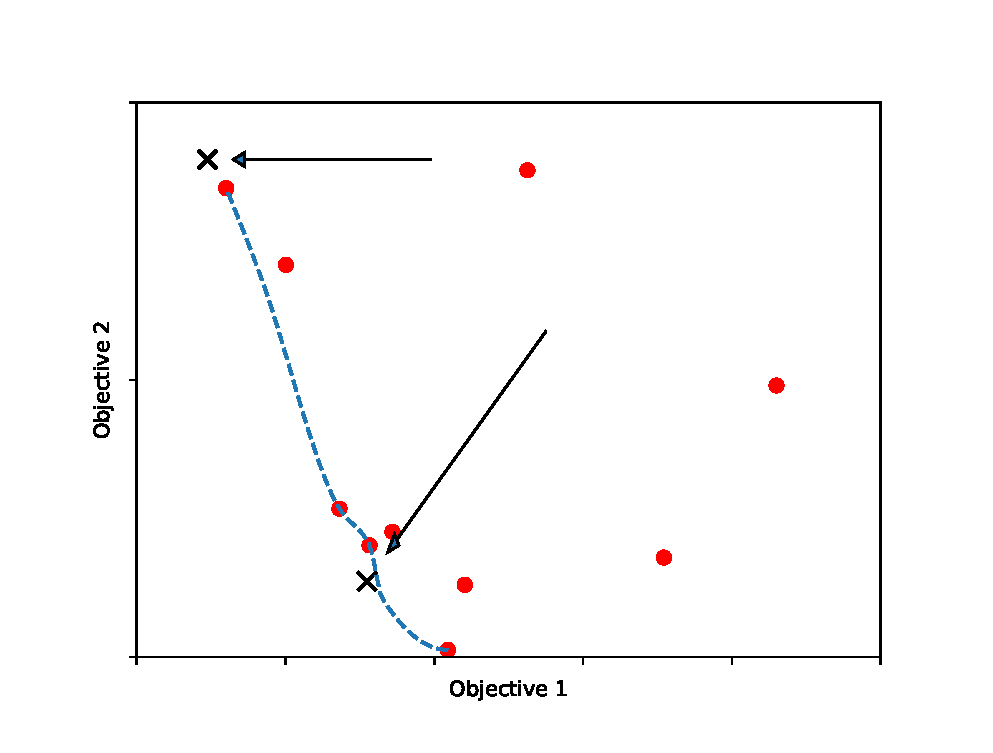
\includegraphics[width=0.6\textwidth]{../img/moo_old/tradeoff.eps}%}
\end{center}
\end{column}
\begin{column}{0.2\textwidth}
\begin{center}
%\onslide<3->{
$\xrightarrow{\hspace*{1.5cm}}$%}
\\
\vskip 1.2cm
%\onslide<6->{
$\qquad\qquad\nearrow$\\
{\Huge $\mathcal{C}$}\\
$\nearrow\qquad\qquad$%}
\\
\vskip 1cm
%\onslide<5->{
$\xleftarrow{\hspace*{1.5cm}}$%}
\end{center}
\end{column}
\begin{column}{0.4\textwidth}
\begin{center}
%\onslide<3->{
\includegraphics[width=0.58\textwidth]{../img/probs/cfr-nmr-setup.jpg}%}
\\
\medskip
%\onslide<4->{
$\xdownarrow{0.5cm}$\\
\medskip
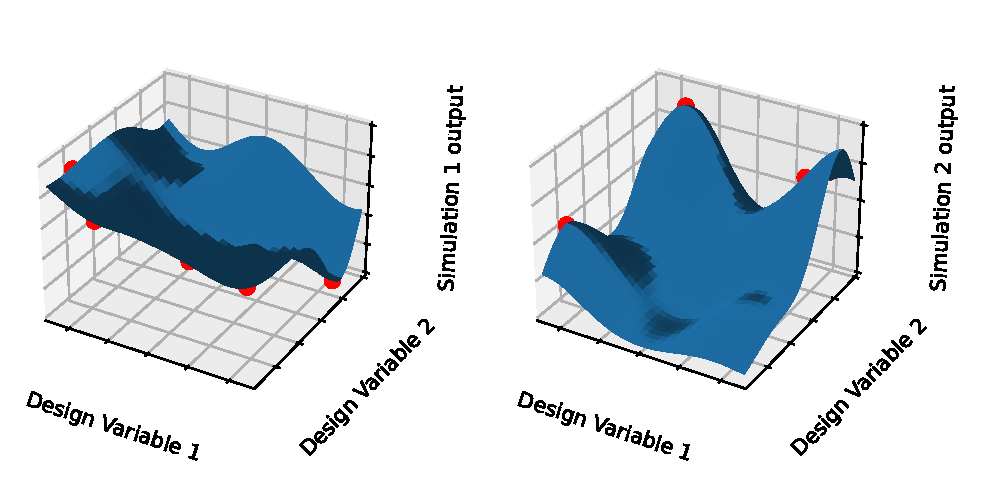
\includegraphics[width=0.9\textwidth]{../img/moo_old/rsm.eps}%}
\end{center}
\end{column}
\end{columns}
\end{frame}

\begin{frame}\frametitle{Challenge 1}
\vfill
\begin{center}
{\Huge \bf
Challenge 1:\\

\bigskip

Mixed vars \& problem types\\
+\\
\medskip

Unusual computing environments
}
\end{center}
\vfill
\end{frame}

\begin{frame}\frametitle{Commercial solutions}
\begin{columns}
%\pause
\begin{column}{0.5\textwidth}
\begin{center}
\includegraphics[width=6em]{../img/probs/linkedin-notifications.png}\\
{\tiny \sl
``Using Bayesian optimization for balancing metrics in recommendation systems''
by Yunbao Ouyang et al.\ on LinkedIn Engineering Blog.\\
}
\end{center}
\end{column}
%\pause
\begin{column}{0.5\textwidth}
\begin{center}
\includegraphics[height=5em]{../img/probs/google-cookies.png}\\
{\tiny \sl
``The makings of a smart cookie''
by Daniel Golovin on Google Research Blog.\\
}
\end{center}
\end{column}
\end{columns}
\begin{columns}
%\pause
\begin{column}{0.33\textwidth}
\begin{center}
\includegraphics[width=5em]{../img/probs/ibm-sdl.png}\\
{\tiny \sl
``Accelerating molecular optimization with AI'' by Payel Das et al.\
on IBM Research Blog.\\
}
\end{center}
\end{column}
%\pause
\begin{column}{0.33\textwidth}
\begin{center}
\includegraphics[height=5em]{../img/probs/meta-nas.png}\\
{\tiny \sl
``Optimizing model accuracy and latency using Bayesian multi-objective NAS''
by David Eriksson et al.\ on Meta AI Research Blog.\\
}
\end{center}
\end{column}
%\pause
\begin{column}{0.33\textwidth}
\begin{center}
\includegraphics[height=5em]{../img/probs/microsoft-nas.png}\\
{\tiny \sl
``Archai can design your neural network with state-of-the-art NAS''
by Shital Shah et al.\ on Microsoft Research Blog.\\
}
\end{center}
\end{column}
\end{columns}
\end{frame}

\begin{frame}\frametitle{Commercial solvers}

%\pause

{\large \bf General purpose:} (solver + backend)\\

\bigskip

Google -- OSS Vizier + Pythia backend

{\tiny\it
[5] Song et al.
OSS Vizier: distributed infrastructure and API for reliable and flexible black-box optimization.
In Proc.\ 2022 AutoML-Conf.
}

\bigskip

Meta -- BoTorch + Ax backend

{\tiny\it
[6] Balandat et al.
BoTorch: a framework for efficient monte-carlo Bayesian optimization.
In NeurIPS 2020.
}

\bigskip
%\pause

{\large \bf Special purpose:} (solver + special purpose deployment)\\

\bigskip

IBM -- Querry-based Molecular Optimization (QMO)

{\tiny\it
[7] Hoffman et al.
Optimizing molecules using efficient queries from property evaluations.
Nature Machine Intelligence 4:21--31 (2022).
}

\bigskip

Microsoft -- Archai for NAS

{\tiny\it
[8] Shah et al.
Archai: platform for neural architecture search.
Microsoft Research (Jul, 2022).
}
\end{frame}

\begin{frame}\frametitle{Challenge 2}
\vfill
\begin{center}
{\Huge \bf
Challenge 2:\\

\bigskip

SOA blackbox optimization\\
+\\
\medskip

Exploiting problem structure
}
\end{center}
\vfill
\end{frame}

\begin{frame}\frametitle{SOA in blackbox optimization}
\begin{columns}
\begin{column}{0.5\textwidth}
\begin{center}
%\onslide<2->{
\includegraphics[width=0.7\textwidth]{../img/logos/logo-scipy.png}\\
{\tiny \sl
``Optimization and root finding (scipy.optimize)'' in SciPy v1.10.0 [9].\\
}
%}
\end{center}
\end{column}
\begin{column}{0.5\textwidth}
\begin{center}
%\onslide<3->{
\includegraphics[height=5em]{../img/probs/siam_news_feb_23.jpg}\\
{\tiny \sl
Stochastic dimension reduction explained in this context
by Stefan [10].\\
}
%}
\end{center}
\end{column}
\end{columns}

\bigskip

\begin{center}
%\onslide<4->{
\includegraphics[width=0.3\textwidth]{../img/logos/logo-tao.png}\\
{\tiny \sl
SOS structure can be exploited by DFO solver POUNDERS in TAO [11].\\
}
%}
\end{center}

\vfill

%\onslide<2->{
{\tiny\it
[9] Virtanen et al.
SciPy 1.0: fundamental algorithms for scientific computing in Python.
{\sl Nature Methods 17:261--272 (2020).}\\
}
%}

\medskip

%\onslide<3->{
{\tiny\it
[10] Wild. Optimization and learning with zeroth-order stochastic oracles.
{\sl SIAM News 56(1):1,3 (2023).}\\
}
%}

\medskip

%\onslide<4->{
{\tiny\it
[11] Wild.
Solving derivative-free nonlinear least squares problems with POUNDERS.
{\sl In Advances and Trends in Optimization with Engineering Applications
(2017).}\\
}
%}
\end{frame}

\begin{frame}\frametitle{ParMOO Design Criteria}

{\large
\textbf{Design goals:}}

\medskip

\begin{enumerate}
\item Highly customizable framework for multiobjective RSM
\item Flexible problem types (mixed-variables, constraints, etc.)
\item Easy to use, deploy, and extend (unforeseen use-cases and environments)
\item Solve large-scale problems + exploit structure and domain knowledge
\end{enumerate}
\end{frame}

\begin{frame}\frametitle{Problem structures}
\begin{center}
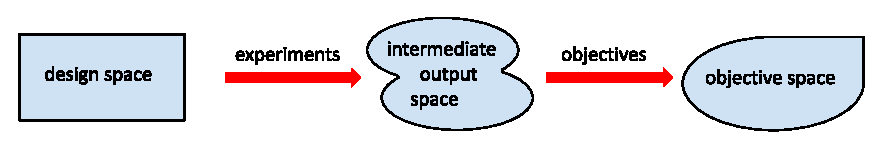
\includegraphics[width=0.9\textwidth]{../img/moo_new/obj-sim-des-space.eps}
\end{center}
\begin{columns}
\begin{column}{0.5\textwidth}
%\pause
\textbf{Least-squares structure:}

\medskip

{\large
$$
{\color{blue} h_i(x, S(x)) = \sum_{j \in N_i} \big({\color{red}S_j(x)}\big)^2}
$$

where each ${\color{blue} N_1, \ldots, N_o}$ is an index set.
}

\bigskip

Increases order of approximation $\Rightarrow$
increases order of convergence

\end{column}
\begin{column}{0.5\textwidth}
%\pause
\textbf{Heterogeneous MOOPs:}

{\large
\begin{align*}
{\color{red} h_1(x, S(x)) = S_1(x)}\\
{\color{blue} h_2(x, S(x)) = \|x \|^2}
\end{align*}
}

Use expensive surrogate models for {\color{red} $h_1$} (i.e.,
{\color{red} $S_1$}) but not for {\color{blue} $h_2$}

\end{column}
\end{columns}
\end{frame}

\begin{frame}[fragile]\frametitle{Sample code}
  \lstset{style=python}
  \lstinputlisting{quickstart.py}
\end{frame}

\begin{frame}\frametitle{ParMOO Release}

\begin{center}
\includegraphics[width=0.4\textwidth]{../img/logos/logo-parmoo.png}
\end{center}

\begin{columns}
\begin{column}{0.7\textwidth}

Written in {\tt Python}

\bigskip

Version 0.2.0 is now available on
available on {\tt pip}, {\tt conda-forge}, and {\tt GitHub}

\bigskip
\bigskip
\url{https://github.com/parmoo/parmoo}

\bigskip

\url{https://parmoo.readthedocs.io}
\end{column}
\begin{column}{0.2\textwidth}
\begin{center}
\includegraphics[width=0.6\textwidth]{../img/logos/logo-py.png}

\bigskip

\includegraphics[width=0.25\textwidth]{../img/logos/logo-gh.png}
$\quad$
\includegraphics[width=0.35\textwidth]{../img/logos/logo-conda.png}
\end{center}
\end{column}
\end{columns}

\bigskip
\bigskip

{\tiny
[15] Chang and Wild.
ParMOO: A Python library for parallel multiobjective simulation optimization.
{\sl JOSS 8(82):4468 (2023).}
}

\end{frame}

\section{Initial Results + Optimizer Stalling}

\begin{frame}\frametitle{Example 1: Material Manufacturing with ParMOO}
Choose optimal settings for material manufacturing in a
continuous flow reactor (CFR)

\bigskip

We know how to make a desired material, need to produce at scale:

\begin{enumerate}
\item {\color{green} \bf Maximize the product} (battery electrolyte: TFML)
\item Can increase temperature to {\bf \color{red} reduce reaction time}
\item Too much heat activates a side reaction; need to
{\bf \color{blue} minimize unwanted byproduct}
\end{enumerate}

\bigskip
\begin{columns}
\begin{column}{0.5\textwidth}
Challenges:

\begin{itemize}
\item Mixed variable types
\item Heterogeneous objectives
\item Must send experiments to run on CFR
\end{itemize}
\end{column}
\begin{column}{0.5\textwidth}
  {\small
  {\sl Design vars and bound constraints}

  \smallskip

      \begin{tabular}{c|cc}
      Parameter & LB & UB \\
      \hline
       Temp (deg C) & 40 & 150 \\
       Reaction time (secs) & 60 & 300 \\
       Equivalence ratio (N/A) & 0.9 & 2 \\
      \hline
       Solvent (categorical) & $\quad$2 & lvls \\
       Base (categorical) & $\quad$2 & lvls \\
  \end{tabular}
  }
\end{column}
\end{columns}
\end{frame}

\begin{frame}\frametitle{CFR Optimization with ParMOO}

\begin{columns}
\begin{column}{0.5\textwidth}

\medskip
Extend {\tt MOOP} class to send/receive experiment data
using {\tt MDML} library (Apache Kafka)

\medskip
Used embeddings to represent
categorical variables

\medskip
Modeled Product/Byprod as sims and reaction time using ID
mapping from input

\begin{center}
\includegraphics[width=0.5\textwidth]{../img/probs/cfr-nmr-setup.jpg}\\
\end{center}
\end{column}
\begin{column}{0.5\textwidth}
\begin{center}
Ran to convergence and used data to create a surrogate problem
for future study\\

\bigskip

\includegraphics[width=0.6\textwidth]{../img/moo_new/cfr_pareto_front.png}\\
\end{center}
\end{column}
\end{columns}

\vfill

{\tiny\it
[17] Chang et al.
A framework for fully autonomous design of materials via multiobjective optimization and active learning: challenges and next steps.
In {\sl ICLR 2023, Workshop on ML4Materials}.\\
}

\end{frame}

\begin{frame}{CFR Optimization Results}

\begin{columns}
\begin{column}{0.55\textwidth}
\begin{itemize}
\item 5 mixed-type design variables (including reaction time)
\item 50-pt Latin hypercube design-of-experiments
\item Fit {\bf global} Gaussian RBF surrogate on 2 simulation outputs
\item {\color{blue}3rd obj is identity mapping of reaction time}
\item 3 $\varepsilon$-constraint scalarization functions
\item Multi-start L-BFGS-B global optimization of scalarized objectives
\item {\color{red}Compared against blackbox implementation: all 3 objectives
modeled with Gaussian RBFs}
\end{itemize}
\end{column}
\begin{column}{0.45\textwidth}
Ran 30 iterations (batch size 3) after initial DOE\\

\bigskip

\includegraphics[width=\textwidth]{../img/moo_old/cfr_hv1.eps}\\

\bigskip

Notice: structure-exploiting is better early on, then
{\bf stalls out} at the end...

\end{column}
\end{columns}
\end{frame}

\begin{frame}\frametitle{Example 2: Fayans EDF Model Calibration}
Find params $x \in [0, 1]^{13}$ to fit the Fayans model to data $d_i$:
$$
M\left(\xi_{i};x\right) \approx d_{i} \qquad i=1,\ldots, 198
$$

\medskip

ParMOO simulation:
$$
S_{i}(x) = M\left(\xi_{i};x\right) - d_{i},
\qquad i=1,\ldots, 198;
$$

\medskip

\begin{columns}
\begin{column}{0.65\textwidth}
Min SOS across 3 observable classes
\end{column}
\begin{column}{0.35\textwidth}
$$
{\color{blue}F_t = \sum_{i=1}^{m_t}\big({\color{red}S_{t,i}(x)}\big)^2}
$$
\end{column}
\end{columns}

\vfill

{\tiny\it
[16] Bollapragada et al.
Optimization and supervised machine learning methods for fitting numerical physics models without derivatives.
Journal of Physics G 48(2):024001 (2020).\\}
\end{frame}

\begin{frame}\frametitle{Fayans Solution with ParMOO}
\begin{columns}
\begin{column}{0.55\textwidth}
\begin{itemize}
\item Approximated Fayans residuals with MLP trained on existing dataset
\item Implemented batch-parallel
{\color{blue} structure-exploiting solver in ParMOO}
\begin{itemize}
\item 2000-pt LH design-of-experiments
\item Use {\bf local} Gaussian RBF surrogates to model sim outs
\item SOS structure applied on top of Gauss RBF surrogate outputs
\item Solve 10 randomized $\varepsilon$-constraint scalarizations per batch
\item Solve scalarized problem with a trust-region-constrained
multi-start L-BFGS-B
\end{itemize}
\item Compared against
{\color{red} same solver w/o exploiting least-squares structure}
(Gaussian RBFs fit directly to three objective values)
\end{itemize}
\end{column}
\begin{column}{0.45\textwidth}
Ran for 800 iterations (10K sim evals)\\

\bigskip

\includegraphics[width=\textwidth]{../img/moo_old/fayans_hv1.eps}\\

\bigskip

Structure-exploiting is better at small budgets, but {\bf stalls} out...
\end{column}
\end{columns}
\end{frame}

\begin{frame}\frametitle{Two different problems, same issue...}
\begin{columns}
\begin{column}{0.5\textwidth}
\includegraphics[width=\textwidth]{../img/moo_old/cfr_hv1.eps}
\end{column}
\begin{column}{0.5\textwidth}
\includegraphics[width=\textwidth]{../img/moo_old/fayans_hv1.eps}
\end{column}
\end{columns}
\begin{columns}
\begin{column}{0.5\textwidth}
\begin{itemize}
\item Mixed-variable problem
\item Extremely limited budget
\item Heterogeneous objectives
\item Global Gaussian RBF modeling
\end{itemize}
\end{column}
\begin{column}{0.5\textwidth}
\begin{itemize}
\item Continuous optimization problem
\item 13 vars, 3 objs, healthy budget
\item Nonlinear least-squares
\item Local RBF (trust-region method)
\end{itemize}
\end{column}
\end{columns}
\end{frame}

\begin{frame}{What happened?}

\pause
\bigskip

Many months of debugging and testing...

\pause
\bigskip

Finally tried centering response values at 0 before
fitting surrogate...

\pause
\bigskip

{\bf Fixed!}\\
\begin{columns}
\begin{column}{0.5\textwidth}
\includegraphics[width=\textwidth]{../img/moo_new/cfr_hv1.eps}
\end{column}
\begin{column}{0.5\textwidth}
\includegraphics[width=\textwidth]{../img/moo_new/fayans_hv1.eps}
\end{column}
\end{columns}
\end{frame}

\begin{frame}\frametitle{Comparison}
\begin{columns}
\begin{column}{0.5\textwidth}
\includegraphics[width=0.8\textwidth]{../img/moo_old/cfr_hv1.eps}
\end{column}
\begin{column}{0.5\textwidth}
\includegraphics[width=0.8\textwidth]{../img/moo_old/fayans_hv1.eps}
\end{column}
\end{columns}
\begin{columns}
\begin{column}{0.5\textwidth}
\includegraphics[width=0.8\textwidth]{../img/moo_new/cfr_hv1.eps}
\end{column}
\begin{column}{0.5\textwidth}
\includegraphics[width=0.8\textwidth]{../img/moo_new/fayans_hv1.eps}
\end{column}
\end{columns}

\vfill

{\tiny\it
[12]
Chang and Wild.
Designing a framework for solving multiobjective simulation optimization problems.
ArXiv preprint 2304.06881 (2023).
}
\end{frame}

\section{Deep-dive into RBFs and Connection to Bayesian optimization}

\begin{frame}\frametitle{Equivalence between Gaussian RBFs and GPs}
For both Gaussian RBFs and (traditional) Gaussian process mean-function:
$$
{\hat F}_{RBF}(x) =
\omega^\top \left[ \begin{array}{c}
e^{-\|x_1 - x\|^2/\sigma}\\
e^{-\|x_2 - x\|^2/\sigma}\\
\vdots\\
e^{-\|x_n - x\|^2/\sigma}
\end{array} \right]
$$
\pause
where
$ A \omega = y $
and 
$$
A = 
\left[
\begin{array}{cccc}
1 & e^{-\|x_1 - x_2\|^2/\sigma} & \ldots & e^{-\|x_1 - x_n\|^2/\sigma} \\
e^{-\|x_2 - x_1\|^2/\sigma} & 1 & \ldots & e^{-\|x_2 - x_n\|^2/\sigma} \\
\vdots & \vdots &  & \vdots \\
e^{-\|x_n - x_1\|^2/\sigma} & e^{-\|x_n - x_2\|^2/\sigma} & \ldots & 1 \\
\end{array}
\right]
\qquad
y = 
\left[
\begin{array}{c}
F(x_1) \\
F(x_2) \\
\vdots \\
F(x_n) \\
\end{array}
\right]
$$

\end{frame}

\begin{frame}\frametitle{RBF/GP Conditioning and Accuracy}
$$
A = 
\left[
\begin{array}{cccc}
1 & e^{-\|x_1 - x_2\|^2/\sigma} & \ldots & e^{-\|x_1 - x_n\|^2/\sigma} \\
e^{-\|x_2 - x_1\|^2/\sigma} & 1 & \ldots & e^{-\|x_2 - x_n\|^2/\sigma} \\
\vdots & \vdots &  & \vdots \\
e^{-\|x_n - x_1\|^2/\sigma} & e^{-\|x_n - x_2\|^2/\sigma} & \ldots & 1 \\
\end{array}
\right]
$$
\begin{itemize}
\pause \item As we optimize, data points cluster
\pause \item As $\|x_i - x_j\| \rightarrow 0$, $A \rightarrow$ singularity
\pause \item Decrease the shape parameter $\sigma$ to keep $A$ nonsingular
\pause \item Descreasing $\sigma$ restricts the support of ${\hat F}_{RBF}$
\begin{itemize}
\pause
\item With 0-prior, optimizer will be driven to low-support regions
\item With GP, uncertainty will be maximal in low-support regions (will drive Bayesian optimization to behave similarly?)
\end{itemize}
\pause \item ``Uncertainty principle'' -- for imbalanced datasets, cannot
have accuracy and solvability when working with RBF-like models
\end{itemize}
\end{frame}

\begin{frame}\frametitle{Big Question}

\begin{center}

{\large \bf
Does Bayesian optimization stall out for structure-exploiting solvers?
}

\pause
\bigskip

{\large \bf
How to even check something like this?
}

\end{center}

\end{frame}

\section{Comparison with Bayesian optimization}

\begin{frame}\frametitle{Implemented Bayesian Optimization in ParMOO}

To check, we implemented Bayesian optimization in ParMOO

\bigskip

\begin{itemize}
\pause\item Structure-exploiting Bayesian optimization is hard, {\bf don't try this at home}
\pause\item When you compose GPs (from simulation outputs) into nonlinear objectives, the posterior depends on the function
\begin{itemize}
\item May or may not be iid
\end{itemize}
\pause \item I monte carlo integrated to evaluate expected-improvement in the $\varepsilon$-constraint scalarization
\begin{itemize}
\item It's very expensive
\end{itemize}
\pause\item Tools like BoTorch are really cool and important
\end{itemize}
\end{frame}

\begin{frame}\frametitle{Bayesian optimization of CFR problem}
\begin{itemize}
\item 5 mixed-type design variables (including reaction time)
\item 50-pt Latin hypercube design-of-experiments
\item Fit {\bf global} Gaussian RBF surrogate on 2 simulation outputs
\item {\color{blue}3rd obj is identity mapping of reaction time}
\item {\color{red}Compared against blackbox implementation: all 3 objectives
modeled with Gaussian RBFs}
\item {\color{green}3 EI of $\varepsilon$-constraint acquisition functions}
\item {\color{green}Monte carlo integration of 2 Gaussian sim outs}
\item {\color{green}Multi-start GPS for global optimization of scalarized objectives}
\end{itemize}

\bigskip

$^*${\color{green} Green highlight} = changes made from before
\end{frame}

\begin{frame}\frametitle{References}

{\tiny\it

[5] Song et al.
OSS Vizier: distributed infrastructure and API for reliable and flexible black-box optimization.
In Proc.\ 2022 AutoML-Conf.

\medskip

[6] Balandat et al.
BoTorch: a framework for efficient monte-carlo Bayesian optimization.
In NeurIPS 2020.

\medskip

[7] Hoffman et al.
Optimizing molecules using efficient queries from property evaluations.
Nature Machine Intelligence 4:21--31 (2022).

\medskip

[8] Shah et al.
Archai: platform for neural architecture search.
Microsoft Research (Jul, 2022).

\medskip

[9] Virtanen et al.
SciPy 1.0: fundamental algorithms for scientific computing in Python.
{\sl Nature Methods 17:261--272 (2020).}

\medskip

[10] Wild. Optimization and learning with zeroth-order stochastic oracles.
{\sl SIAM News 56(1):1,3 (2023).}

\medskip

[11] Wild.
Solving derivative-free nonlinear least squares problems with POUNDERS.
{\sl In Advances and Trends in Optimization with Engineering Applications
(2017).}

\medskip

[12]
Chang and Wild.
Designing a framework for solving multiobjective simulation optimization problems.
ArXiv preprint 2304.06881 (2023).

\medskip

[15] Chang and Wild.
ParMOO: A Python library for parallel multiobjective simulation optimization.
{\sl JOSS 8(82):4468 (2023).}

\medskip

[16] Bollapragada et al.
Optimization and supervised machine learning methods for fitting numerical physics models without derivatives.
Journal of Physics G 48(2):024001 (2020).

\medskip

[17] Chang et al.
A framework for fully autonomous design of materials via multiobjective optimization and active learning: challenges and next steps.
In {\sl ICLR 2023 Workshop on ML4Materials}.

}
\end{frame}

\begin{frame}\frametitle{Resources}
\begin{center}
{\large
GitHub: {\tt github.com/parmoo/parmoo}\\
Docs: {\tt parmoo.readthedocs.io}\\
PyPI: {\tt pip install parmoo}\\
Conda: {\tt conda install --channel=conda-forge parmoo}}

\bigskip
\bigskip

E-mail: {\tt tchang@anl.gov}\\
E-mail: {\tt parmoo@mcs.anl.gov}\\
\bigskip
\bigskip
{\sl Chang and Wild. JOSS 8(82):4468 (2023)}\\

\vfill

{\tiny This material is based upon work supported by the U.S. Department of Energy, Office of Science, Office of Advanced Scientific Computing Research, SciDAC program under contract number DE-AC02-06CH11357.\\}

\end{center}
\end{frame}

\end{document}
